\documentclass{article}
\usepackage[utf8]{inputenc}
\usepackage{listings}
\usepackage{float}
\usepackage{natbib}
\usepackage{graphicx}
\usepackage{amssymb}
\usepackage{amsmath}
\usepackage{amsthm}
\usepackage{mathtools}
\usepackage{listings}
\usepackage{color}
\usepackage{hyperref}
\usepackage{ amssymb }
\usepackage{musicography}
%\usepackage[linesnumbered,ruled]{algorithm2e}
\usepackage{algorithm}
\usepackage{algpseudocode}
\usepackage{physics}
\usepackage{fancyhdr}
\NeedsTeXFormat{LaTeX2e}
\ProvidesPackage{quiver}[2020/11/27 quiver]
\newtheorem{theorem}{Theorem}[section]
\newtheorem{corollary}{Corollary}[theorem]
\newtheorem{lemma}[theorem]{Lemma}

% `tikz-cd` is necessary to draw commutative diagrams.
\RequirePackage{tikz-cd}
% `calc` is necessary to draw curved arrows.
\usetikzlibrary{calc}
% `pathmorphing` is necessary to draw squiggly arrows.
\usetikzlibrary{decorations.pathmorphing}

\definecolor{dkgreen}{rgb}{0,0.6,0}
\definecolor{gray}{rgb}{0.5,0.5,0.5}
\definecolor{mauve}{rgb}{0.58,0,0.82}

\tikzset{curve/.style={settings={#1},to path={(\tikztostart)
    .. controls ($(\tikztostart)!\pv{pos}!(\tikztotarget)!\pv{height}!270:(\tikztotarget)$)
    and ($(\tikztostart)!1-\pv{pos}!(\tikztotarget)!\pv{height}!270:(\tikztotarget)$)
    .. (\tikztotarget)\tikztonodes}},
    settings/.code={\tikzset{quiver/.cd,#1}
        \def\pv##1{\pgfkeysvalueof{/tikz/quiver/##1}}},
    quiver/.cd,pos/.initial=0.35,height/.initial=0}

% TikZ arrowhead/tail styles.
\tikzset{tail reversed/.code={\pgfsetarrowsstart{tikzcd to}}}
\tikzset{2tail/.code={\pgfsetarrowsstart{Implies[reversed]}}}
\tikzset{2tail reversed/.code={\pgfsetarrowsstart{Implies}}}

\lstset{frame=tb,
  language=Scala,
  aboveskip=3mm,
  belowskip=3mm,
  showstringspaces=false,
  columns=flexible,
  basicstyle={\small\ttfamily},
  numbers=none,
  numberstyle=\tiny\color{gray},
  keywordstyle=\color{blue},
  commentstyle=\color{dkgreen},
  stringstyle=\color{mauve},
  breaklines=true,
  breakatwhitespace=true,
  tabsize=3
}
\newcommand{\colim}{\operatorname{colim}}

\newcommand\rightthreearrow{%
        \mathrel{\vcenter{\mathsurround0pt
                \ialign{##\crcr
                        \noalign{\nointerlineskip}$\rightarrow$\crcr
                        \noalign{\nointerlineskip}$\rightarrow$\crcr
                        \noalign{\nointerlineskip}$\rightarrow$\crcr
                }%
        }}%
}

\newcommand\righttwoarrow{%
        \mathrel{\vcenter{\mathsurround0pt
                \ialign{##\crcr
                        \noalign{\nointerlineskip}$\rightarrow$\crcr
                        \noalign{\nointerlineskip}$\rightarrow$\crcr
                }%
        }}%
}

\graphicspath{ {./images/} }

\title{2MEME}
\author{Wyatt L. Meldman-Floch}
\date{11/27/2023}
\setlength{\parskip}{1em}

\fancyhf{}
\renewcommand{\headrulewidth}{0pt}
\fancyfoot[c]{}
\fancypagestyle{FirstPage}{
\lfoot{\copyright2023 Wyatt Meldman-Floch} 
}

\begin{document}
\maketitle

\begin{abstract}
2MEME, a reputation model for p2p systems based on peer metadata and cryptographically secure hashes, is presented. It is dynamic, not relying on a set of trusted peers, and rotates the most accessible peers as leaders: those with the minimal entropy rate relative to all peers, or peers producing the most correct information. The core application and focus is optimizing consistency of a multi-layered consensus protocol, achieving Asynchronous Byzantine Fault Tolerance.

\end{abstract}

\tableofcontents

\setcounter{secnumdepth}{0}

\section{Forward}
\thispagestyle{FirstPage}
The following is a solution of a long standing goal in the crypto ecosystem: creating a consensus process that rewards good behavior and mitigates bad behavior, directly. A fundamental problem with existing blockchain technology is that while it aims to achieve decentralization, both the logic and the algorithmic complexity of existing consensus protocols limit the group of individuals who can mine to a small few. A core requirement to make mining accessible to the average person i.e. run on consumer hardware, is to remove the barrier to entry caused by proof or work which requires expensive hardware or proof of stake which requires substantial financial capacity. A consensus protocol that's accessible to the average consumer will make mining a viable alternative to application hosting and monetization of the web as a whole; as well as create new systems of governance that can engage the average person to participate in directly. It turns out that the solution is to provide incentives to nodes for acting in a way that optimizes their consistency (the C in the CAP theorem) and penalizes for network partitions.

2MEME is partially named because it incorporates two memetic concepts into a sybil attack resistance model: relative entropy or information gain, defined by the commonality of each node's state and node influence, which calculates how adherent each node's behavior is relative to the total set of nodes' behavior. The adherence to a performance 'meme' is how rewards are generated, essentially paying nodes for being the most consistent (common state with the whole) and the adherence to an influence 'meme' is how sybil behavior is determined; nodes that are not sybil follow a noisy distribution, while sybil nodes are identified by a strong signal. It's also sort of the sequal to an older approach to solving the above problem, which was called MEME. MEME differs from 2MEME in that it didn't use information gain as the feature space, opting to try and define a classifier and passing in a covariance matrix into the self-avoiding walk below, then normalizing using entropy of the walk output. That older version, which became Constellation's PRO, relied on a set of pre-trusted peers, which is a similar approach applied by most DAG protocols, but essentially became a federated proof of authority. The improvement, which became 2MEME, stems from application of a previous work, still in preprint, called the Generative Calculus, and the algorithm/results here will be used to expand upon generative calculus in that paper. 2MEME's implementation within the reality protocol is completely permission-less, but it could be re-written for a permissionned environment which would result in a potential improvement on fault tolerance (at least algorithmically, as it removes a serial state transition).

Note: This work is in pre-print and as of now a first-draft. The pseudocode sections aren't exactly the syntax I wanted but the pseudocode library is getting the job done. Also, I'm still working on formatting the surface plots in the results section. They're actually rendered in 3d, so if you run the code yourself\footnote{https://github.com/reality-foundation/reality/blob/enable\_model/simulation\_data/surface\_plot.py} you can re-orient to get different views of the surfaces.

\section{Introduction}
For a distributed system to maintain consistency, it needs to optimize information gain and minimize discrepancies. One set of approaches rely on trust or reputation models to mitigate potentially conflicting updates from untrusted peers. There are many approaches to solving reputation problems in p2p networks. The most famous is Eigentrust, and there are many expansions upon the base framework, such as Honestpeer and Powertrust. Due to the curse of dimensionality, they all employ some type of random walk to explore the search space of transitive trust between nodes, calculating a probability distribution such as via Monte-Carlo integration to generate probabilistic trust scores of all peers. These expansions typically focus on finding new features or representations of trust, such as in Deepwalk or Node2vec, which create an embedding of social data to normalize the edge weights of the peer graph.

This paper follows a similar approach using entropy or disorder across peer behavior and is specifically applied to a dag-based multi-layered consensus protocol. Whereas many approaches such as Eigentrust require a seed or whitelist of authority nodes to base trust upon, this is insufficient when requiring decentralization such as for distributed consensus networks like cryptocurrencies. 2MEME circumvents this by determining correctness without pre-trusted peers, allowing nodes to join and leave and preventing centralized control over consensus.

The core of the algorithm extends from the principle of maximal entropy, however applied in reverse. The maximum entropy principle states that new information added to a system increases disorder relative to the previous state of that system, proportional to novel information added. However, in the system architecture described below, the data structures themselves optimize the spread of incoming data via rumor based gossip such that discrepancies between peer state form cliques representing potential network partitions.

Periodically, a self avoiding random walk is performed on a graph of nodes representing peers, with the edges representing a vector of the entropy rate calculated between data processed by each peer and the total set of data processed. The model chooses correct nodes according to a 'node influence metric' based on 'availability', which is defined as the most strongly linked nodes; ranking the peers/nodes by how similar their behavior is relative to the total set of nodes' behavior.

Another goal of 2MEME is to improve upon PRO models by handling node 'churn' in a permissionless environment, achieving 'elasticity' comparable to elastic infrastructure like Elasticsearch and Elastic Map Reduce, while still maintaining objective decentralization by operating without potentially fraudulent human input.

\section{System Architecture}
The system considered here consists of a two layer consensus protocol, with two separate consensus processes, L1 and L0, directly influencing each other. Future work incorporating more consensus layers can be formulated using the Poincare Protocol and Protocol Topology specified in Blockchain Cohomology\footnote{Meldman-Floch, Wyatt, ``Blockchain Cohomology: Sec 23' \\ http://ceur-ws.org/Vol-2478/paper2.pdf}.

L1 peers perform a federated consensus of $O(\sum peers/3) \equiv O(n)$ complexity, converging on the state of each peer’s state cache. The contents of each state cache is a ledger of Addresses and collection of Transactions: data structures performing the transfer of a numerical amount (tokens) from one Address to another Address. Each Address has an associated linked list formed out of Transactions sent from this Address. The links are recursive cryptographic signature hashes between each sequential transaction at a discrete Ordinal.

Periodically, as each L1 node reaches the limit of its mempool or in response to a timed trigger, they initiate a consensus process, acting as an ‘owner’ peer, which selects two ‘facilitator’ peers to share its state cache with. The two facilitator peers also share their state cache with each other, then back to the owner, and then to all other peers. The output of this process is a data structure, signed by the owner and facilitators, called a ‘block’ which consists of each peer’s state cache data and two ‘parent edges’ called Tips, which are hashes of previous blocks; the end result is a triangle, where two corners are tips and the third is the new block. This can be conceptualized as a ‘triangulation of state’ which forms a forward arrow of time out of parallel-process state transition data. This is realized as a data structure called the ‘Data Dependency Graph’ which is a directed acyclic graph of blocks with two parent edges, and three dimensions; namely, height, width and depth. 

\begin{figure}
\centering
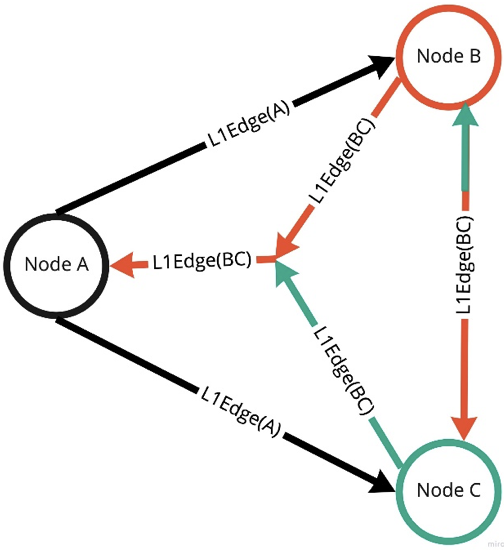
\includegraphics[width=0.5\textwidth, height=0.5\textwidth]{L1-hylo}
\caption{L1 consensus}
\end{figure}

These blocks constitute a directed acyclic graph called the Data Dependency Graph and their contents are validated by the L0, which updates the ledger of Addresses with valid Transactions. Both of these have a poset topology, from which the forward arrow of time can be constructed out of parallel events. Each block is then spread across all L1 and L0 peers via rumor based gossip, so that they can be used as ‘Tips’ to form edges between old and new blocks.

\begin{algorithm}
\caption{L1 consensus algorithm}\label{alg:cap}
\begin{algorithmic}

\State $n \gets N \in \mathbb{N}$ \Comment{these are L1 nodes}
\State $n.mempool \equiv \{ $Transactions$ \}$
\State $n.mempool.size, n.mempool.triggersize \in \mathbb{N}$
\State $n.mempool.size, n.mempool.triggersize \gets n$ 
\State $received Owner Proposal(): bool$
\State $recieved Facilitator Proposal(): bool$
\State $isOwnerPeer(n): bool$
\While{True}
	\If{$n.mempool.size \geq n.mempool.t$}
		 \State Create owner proposal
		 \State Send to 2 L1 peers
		 \State Validate responses
		 \State Form block and gossip to all L1 and L0 nodes
		
	\ElsIf{$received Owner Proposal()$}
			\State Sign and send proposal made from current node's mempool to other Facilitator peer
		
	\ElsIf{$received Facilitator Proposal()$}
		\If{$isOwnerPeer$}
			\State Ensure both Facilitator proposals are equal
			\State sign and send block (made of all 3 mempools) to other all L1 and L0 nodes
		\Else
			\State Send Facilitator proposal to Owner
		\EndIf
	\EndIf
\EndWhile

\end{algorithmic}
\end{algorithm}

Tips and Facilitators are selected using a pure function that seeks to maximize the area (in terms of dimensions: height, width and depth) thus increasing the potential parallelism by enforcing consistency across all peers. L1 nodes are pruned according to an entropy calculation by L0 nodes on the blocks they create; each block is created deterministically according to the total set of tips and peers, deviations from this result low rewards and in low trust. L1 trust scores are then normalized between 1 and -1 with low trust outliers being removed and addresses temporarily blacklisted.

Data contained in the L0 peer's mempool, consisting of L1 blocks, is spread amongst L0 peers via rumor based gossip with $O(log(\sum peers))$ complexity, converging the state of each peer to the union of all peers'. Periodically, as the Data Dependency Graph reaches new heights or on a timed trigger in case of low network traffic, each L0 peer proposes a Snapshot to its L0 peers using rumor based gossip. The contents of these Snapshots are L1 blocks, and a parent reference, formed out of recursive cryptographic signatures, to the peer’s previous Snapshot proposal. This forms a sequential/poset topology for L0 peer proposals like for Addresses. At each ‘height’ step, one proposal is selected from the set of all proposals, deemed the Majority Snapshot. The Majority Snapshot is chosen as the count of occurrences within the set of proposals, multiplied by the total  node influence or cumulative sum of trust scores of each peer that proposed it. 
	
Periodically, at an interval multiple of snapshot height called the 'height-diff' interval, the L0 nodes cycle between ‘active’ and ‘passive’ states. 'Active' nodes actively perform consensus, 'passive' nodes gather final snapshots and index into a database (block explorer). The total number of 'active' L0 nodes is equal to $\sqrt{\sum peers}$, thus the total complexity for ledger state convergence (known as finality time) is $O(\sqrt{\sum peers}^2) + O(log(n)= O(n) + O(log(n))$. Peers are cycled at each interval according to a deterministic locality sensitive hash function applied to the last snapshot hash and all the L0 peer addresses that have not been identified as Sybil; a node's probability of selection is also influenced by the amount of tokens in the address of the node, however the amount does not affect the outcome of consensus (which constitutes proof of stake). Rewards for each round are proportional to the cumulative sum of information gain reported by L0’s peers and low trust outliers are blacklisted temporarily.

In both L0 and L1, a 'double spend' or submission of invalid data as valid, with the attempted result being the attribution of new tokens to some Address, the node Address's balance is reduced to 0 in a process known as 'slashing'. It is also worth noting that, as shown via recursive tip structure, there is no fault tolerance due to latency, thus it's fault tolerance is asynchronous and achieves Asynchronous Byzantine Fault Tolerance.

\begin{algorithm}
\caption{$L \Omega$}\label{alg:cap}
\begin{algorithmic}
\State $h, i \in \mathbb{N}$
\State $H \ggg  i$
\State $h \gets H$
\State $n \gets N$ \Comment{these are $L\Omega$ nodes}
\State $n.mempool \equiv \{ $Snapshots$ \}$
\State $n.mempool.size, n.mempool.triggersize, n.peers.active, n.peers.passive \in \mathbb{N}$
\State $n.mempool.size, n.mempool.triggersize, n.peers.active, n.peers.passive \gets n$ 
\State $h.signatureChain \leq n.peers.active$ 
\State $isActive(n): bool$
\State $invalidSnapshot(h): bool$
\State $notUnique(h): bool$

\For{$h \gets H$}
	\If{$invalidSnapshot(h)$}
		\State Slash address value for all signatories on h
		\State Remove invalid signatories from n.peers.active
		\If{$n.peers.active - invalid signatories == 0$}
			\State Recalculate active peers from previous snapshot and previous set of inactive peers
			\State Gossip new active state to all subscribers (including L1 and client apps)
		\EndIf
		
	\ElsIf{$notUnique(h)$}
		\If{$h.signatureChain < n.peers.active $}
			\State Initiate health check/removal on missing peer ids
		\EndIf
		\State Choose h with highest $\sum_n{score(n)}$

	\ElsIf{$0 \equiv h \bmod{i} == 0$}
    			\State Calculate new active peers
			\If{$isActive(n)$}
				\State Initiate active L0 process with other active peers
			\EndIf
	\ElsIf{$0 \equiv h \bmod{i-1} == 0$}
    		\State Send 
		
	\ElsIf {$\not isActive(n) \& \not invalidSnapshot(h)$}
	    		\State Gossip join requests, Snapshots
			\State Submit data to Downloading nodes
			\State Process ledger state requests
		
	\EndIf
\EndFor
\end{algorithmic}
\end{algorithm}

Finally, there is a meta-process running on all L0 nodes (both active and passive), which acts as a block explorer in addition to validating L0 snapshots and curating the list of all peers, namely the L$\Omega$. All active L0 peers need to sign the result of consensus (form a signature chain), which enforces convergence before sending to the larger $L\Omega$ network, but also creates a record of divergence (either malicious or not) and the nodes that diverged. If this happens, a health check is performed, essentially asking for the missing data; if it is not received, then the unresponsive peers are removed and consensus continues. In order to maintain a consistent peer list, new peer requests are gossiped across the active and passive nodes via $L\Omega$ and included in Snapshots.

\subsection{Active Peer Selection}
Active peer selection is performed by a deterministic locality sensitive hash function which operates on a list of peers and chooses equal amounts randomly between two partitions of active nodes; one partition $A$ making up a minimum of $50\%$ of all staked tokens, and the second partition $B$ containing all remaining nodes. It's clear to see that as the network grows it implies that $B \ggg A$ due to token scarcity. While this does provide an advantage for early users/token holders, it mitigates the security risk inherent in horizontally scalable permissionless networks (which get faster as the network grows) while still providing ample possibility for new users (with lower stake) to participate. 


\section{Minimizing the Entropy Rate}
Information gain can be formulated as the reduction of entropy or disorder in a dynamical system and depending on the characteristics of the system, it is calculated in one of many ways. For the purposes of 2MEME, which is formulated for application to consensus networks, it is calculated as a stochastic process.
	A stochastic process is an indexed sequence of random variables that do not need to be independent or identically distributed. In a consensus network, each peer continuously proposes variable state data, converging on an accepted state according to the rules of the consensus algorithm. This state data, in our case called blocks, can be independent or dependent on each other; and the amount of blocks as well as the specific blocks proposed can fluctuate or differ completely. Each block has an indexed order, or in the case of the system architecture above, a poset topology; meaning that they are strictly ordered. Thus these distributed systems fulfill the requirements of a stochastic process and can be modeled as such. While it is possible to apply 2MEME to linear blockchain protocols, it was formulated specifically for use in the system architecture above, with three indices: height, width and depth. The following formulas are specific to this poset topology.
	Consider a set of peers $N = (n_0 …n_i)$, acting as random variables which produce outputs $O = (o_{0,0,0} … o_{h,w,d})$, such that $h<w$ and $w>d$, the system has a strict order given by poset topology. These indices can be reduced to discrete indexes, such that each index, there is a binary value representing each node proposing a specific block or not. This is calculated using following formula\footnote{thm 2.4 'https://math.nd.edu/assets/275279/leblanc\_thesis.pdf'} for joint entropy	
\begin{equation}
H(N) = -\sum_{n_1 \in N_1} \dots \sum_{x_n \in N_n} P(n_1,  \dots, n_N) log_2 [P(n_1, \dots, x_n)]
\end{equation}
	
	the limit of which as h, w, d approaches infinity gives the entropy rate.
If a block index contains each node, then the specific block has entropy of 0. If it contains $|n| < N$, the entropy is $> 0$. Conversely, if nodes propose blocks such that their indices conflict with other proposals, they contribute to the overall disorder in the system. Proposed blocks with valid yet duplicated data, contribute to overall disorder as well. Thus the state with the minimal entropy can be considered the greatest common subset of all proposed blocks, and entropy calculated as deviation from the greatest common subset. Note that in the case of graph partitions that are not within this subset, yet still contain valid data, the data should still be contained within the overall state transition, however the node that only processed it’s lone subset can be considered faulty (potentially Sybil) in terms of consistency and partition tolerance (CAP). In order to promote consistency, a rumor based gossip algorithm propagates blocks, calculating signatures upon them, which then can be used as Tips, to optimize for a maximal subgraph of peers to accept the block and propose it within its Snapshot. This impedes several sybil attacks such as lie and wait and ddos, by attempting to create the longest signature chain as possible, i.e. the largest common subset; nodes attempting these types of attacks are identified via independent subsets and/or invalid blocks.

Finally, the inner product of entropy rates are used to construct a feature space $F$ before passing into the random walk below (first part of 2MEME)

\begin{equation}
F = \sum_N \lambda_N \ket{N_n} \bra{N_n}
\end{equation}

where $\lambda$ is a normalization function that maps the sum to between -1 and 1.

\section {L0 consensus: Permissionless vs Permissioned approaches}
Two algorithms for gathering entropy data are presented below. The key algorithmic difference is the rate and logic for making proposals. 

The first enforces a service level agreement requiring each peer to train its model at the same rate, achieving greater determinism and enabling a token reward model for an open network and preventing nodes' ability to forge scores to manipulate the selection algorithm; by first committing an encrypted hash of their scores to the ledger, then sending the unencrypted scores so peers can calculate the Majority Snapshot. In the batch model, at every snapshot height-diff interval, each peer proposes a new predicted trust vector (scores) within their proposals. They are then used to weight peer proposals for the Majority Snapshot calculation.

\begin{algorithm}
\caption{Batch Algorithm (permissionless): Entropy Rate (Optimal for node rewards/cycling between active and passive nodes)}\label{alg:cap}
\begin{algorithmic}
\State $h, i \in \mathbb{N}$
\State $H \ggg  i$
\State $h \gets H$
\State $n \gets N$ \Comment{these are L0 nodes}
\State $n.mempool \equiv \{ $Blocks$ \}$
\State $n.mempool.size, n.mempool.triggersize \in \mathbb{N}$
\State  $n.mempool.size, n.mempool.triggersize \gets n$ 

\For{$h \gets H$}
	\If{$0 \equiv h \bmod{i-1} == 0 \& n.mempool.size \geq n.mempool.t$}
    		\State $stateSpace = entropy(N)$ \Comment{Entropy rate relative to GCS}
   	 	\State $probabilitySpace = selfAvoidingWalk (state space)$  
   	 	\State Send encrypted $probabilitySpace$ to peers within Snapshot
    		\State Choose proposed snapshots weighted by cumulative sum of scores

	\ElsIf{$0 \equiv h \bmod{i} == 0 \& n.mempool.size \geq n.mempool.t$}
    			\State Send unencrypted $probabilitySpace$ within snapshot to peers
    			\If {$valid(n), \forall n \in N$}
    				\For{$n \gets N$}
   				 	\State Update scores for peers
					 \State Choose Majority Snapshot
					 \State Update active and passive peerlist
				\EndFor
			\EndIf
		
		
	\ElsIf {$n.mempool.size \geq n.mempool.t $}
	    		\State Send snapshot to peers
	    		\State Choose proposed snapshots weighted by cumulative sum of scores
		
		
	\EndIf
\EndFor
\end{algorithmic}
\end{algorithm}

The second, online algorithm, reduces the in-memory cost of running each peer’s model on a deterministic schedule albeit at the loss of determinism that would allow fair selection of validators. It is more suited perhaps to applications that can relax determinism required by an open network to focus on elasticity. The online algorithm periodically gossips predicted trust vectors to peers over the Peer api endpoint (“~/trust”), which are then cached and fed into the TrustManager on a time based periodic interval.

\begin{algorithm}
\caption{Online Algorithm (permisioned): Approximate Entropy Rate (current implementation, optimal for minimal resource usage, training model over shorter periods should help output, spamming results/sybil collusion should be detected by model, good test)}\label{alg:cap}
\begin{algorithmic}
\State $h, i \in \mathbb{N}$
\State $H \ggg  i$
\State $h \gets H$
\State $n \gets N$ \Comment{these are nodes}
\State $n.mempool \equiv \{ $Blocks$ \}$
\State $n.mempool.size, n.mempool.triggersize \in \mathbb{N}$
\State  $n.mempool.size, n.mempool.triggersize \gets n$ 
\State $e = rand(): bool $ \Comment{This is a timed based trigger}
\While{True}
	\If{$n.mempool.size \geq n.mempool.t \&  e == True$}
		 \State $state space = entropy(N)$ \Comment{Entropy rate relative to GCS}
   	 	\State $probabilitySpace = selfAvoidingWalk (state space)$  
	 	\State Send unencrypted scores to peers in Snapshot
	 	\State Update active and passive peerlist
		
	\Else {$n.mempool.size \geq n.mempool.t$}
			\State Send snapshot to peers
			\State Choose Majority Snapshot
	\EndIf
\EndWhile
\end{algorithmic}
\end{algorithm}

\section{Monte Carlo simulation: estimation via self avoiding random walk}
Next a self-avoiding walk is employed to perform community detection, the output of which can be used to calculate availability and node influence\footnote{https://www.sciencedirect.com/science/article/pii/S0378437118304242}. Note, to avoid confusion between a consensus network and graph, nodes are called servers below.

The output of the entropy rate calculation is a graph, with a server’s peers corresponding to nodes and edges as the relative joint entropy between the server and its peers. The edges are a ‘view’ of the performance of each peer relative to itself. This matrix (namely $F = \sum_N \lambda_N \ket{N_n} \bra{N_n}$) is passed to the TrustManager, a background process that performs a self-avoiding random walk across the graph of nodes connected by relative joint entropy and outputs a vector containing a trust score for each node relative to the server hosting running the process (predicted trust). Pseudocode for this and the following methods are omitted due to length, but can be found in the Reality Protocol's codebase\footnote{https://github.com/reality-foundation/reality/tree/enable\_model/modules/sdk/src/\\main/scala/org/tessellation/sdk/infrastructure/trust}.

The self avoiding walk is performed by the method runwalkfeedbacksinglenode, which performs a series of feedback rounds, walking on the input graph and adjusting the edge weights between nodes for each successive round. The total number of feedback cycles are configurable and in general the larger number of cycles has a more accurate output, albeit at the cost of increasing resource intensity. The configurations are batchIterationSize and maxIterations. On each batch iteration a random path length from a random number generator (between 1 and total nodes) is chosen and then passed to the walk. The walk goes through and only walks on positive edges (relative entropy scores are normalized between -1 and 1), keeps track of nodes visited so far, then the sampling function determines the next neighbor to walk on. This is determined according to the normalized probability (via method normalizedPositiveEdges), such that the positive edge subset sum up to one.

As this iterates, transitive trust scores are added, because products of trust are quite small. However, over many iterations they sum, to large numbers which is better for differentiating between scores. The main walk function walk() gets invoked by walkFromOrigin() inside runWalkRaw() which iterates over numIterations, adding up the scores into val walkScores for each node, removing the server’s own. After that function is called, one “batch” has been created. 

Finally there is batch convergence in runWalkBatchesFeedback. This converges when a delta variable, which is just root mean squared error, becomes less than or equal to an epsilon variable, where epsilon is set to 1e-6; i.e the function terminates when scores don’t change between batches by one part in a million. The output of the walk, batchScores, is not normalized, so they are renormalized by the Normalize function between each iteration until convergence.

One difference from similar models is the incorporation of negative scores. After the batches are performed, it explores the negative scores (val negativeScores) of nodes that it trusts (positive outputs of the walk). On the first cycle, the model only reaches nodes with positive transitive trust, which can be considered the most influential servers. These most influential servers are relative to the host server, and the servers they distrust have their scores down weighted. The positive scores and negative scores are added, then weighted by how influential the server proposing these scores is. They are weighted such that its negative edge trust quantity*(influential node’s score/numNegEdges), after that they are all normalized via renormalizeAfterNegative. Output, $P_i^h$ is defined as follows.

Given a source node $i$, suppose it is possible to reach $N_i(h)$ different nodes performing walks of length $h$, departing from $i$. Then we say that $i$ has $N_i$ neighbors at a distance $h$. Each neighbor is reached with a different probability, which is represented by the vector $P_i^h = \{ P_1^{(h)} \dots P_{N_i(h)}^{(h)} \}$ Given $P_i^h$,the accessibility $k_i(h)$, defined below is 
	
	
\begin{equation}
k_(h) = \exp (-\sum_j p^{h}_j log p^{h}_j )
\end{equation}

\section{Classification logic}
Now  that we have a manifold of node influence, we can look for signals between sybil and non-sybil nodes and build a classifier. Pseudocode for the classifier is omitted due to length, but can be found in the Reality Protocol's codebase\footnote{https://github.com/reality-foundation/reality/blob/enable\_model/modules/sdk/src/\\main/scala/org/tessellation/sdk/infrastructure/trust/TrustModel.scala}.

The classifier defined as follows simply looks at the first three principal eigenvectors (those with the largest three eigenvalues), to identify sybil nodes. Its quite possible to improve upon the experimental results using a differential equation solver as provided in Tensorflow \footnote{https://www.tensorflow.org/probability/api\_docs/python/tfp/math/ode} or Pytorch\footnote{https://github.com/rtqichen/torchdiffeq}, which would be able at least incorporate higher order terms and improve distribution fit, if not catch hidden nonlinear signals. As you'll see, the classifier follows steps similar to those in analytically solving systems of differential equations.

First a new vector consisting of the successive diffs, normalized between 0 and 1, between all elements in $P_i^h$ is calculated, namely $d_i^h$ which has $dim(i, h-1)$ then generate a manifold from direct sum with itself:

\begin{equation}
d_i^h \oplus d_i^h
\end{equation}

calculate the principal components (eigenvectors sorted by highest eigenvalue), $\lambda_1, \lambda_2 ,\lambda_3$ as well the 'max plane' $p_i$, similar to the 'top hat' in signal/fourier analysis which is an index range in $d_i^h$ with flat values (not perfectly flat, all diffs are within a threshold of the mean $\mu$ or a minimum of 0.1), the 'right bias' $b_r$ and 'left bias' $b_l$ which are the ration of total sum of values to the left of $p_i$ divided by total scores and  total sum of values to the right of $b$ divided by total scores respectively. Finally consider 'population diffs' 

\begin{equation}
\lambda_{pop} = 1-(\lambda_{i-left}/\lambda_{i-right})
\end{equation}
where $1-(\lambda_{i-left}/\lambda_{i-right})$  are the population or number of nodes contained within biases calculated from each of the principal eigenvalues.

Now, there are five scenarios to determine non-sybil nodes: first if the max plane makes up over $20\%$ of the distribution and either biases are less than $90\%$ of the distribution, return the biases as non-sybil nodes. Second, if either the absolute value of the ratio of mean to population variance is less than $1x10^{-17}$ or the difference between the absolute value of the first principal component and the  absolute value of the second principal component is greater than the population standard deviation by $30\%$, return the entire set of $P_i$. Third, if the difference between the principal and second principal eigenvector is greater than the population standard deviation by $20\%$ or the minimum population diff (of all 3) is the population diff of the maximum principal component, then if the difference between the absolute values of the population biases of the principal eigenvalue $|\lambda_{left}| - |\lambda_{right}|$ is greater than the population standard deviation, return the right bias of the max principal component; if only the first condition is true, return the left bias of the max principal component. Next he same logic is then applied for the second and third principal components. 

Finally, if the total non-sybil nodes to be returned are less than $10\%$ of the population ($90\%$ identified as sybil), return the entire set of nodes.

\section{Experimental results}
The following results were generated from a simulation involving 100 node instances. Several simulations were run for various types of attacks, which will be outlined below, and with varying percentages of sybil nodes all acting in unison from $0\%$ to $100\%$ in 20 percent intervals. Each type of attack can be reduced down to sybil nodes reporting scores of themselves or non-sybil nodes according to a distribution i,e low scores for non-sybil or high scores for sybil nodes. In the following visualizations, each attack type occurs on the y axis, the sybil percentage is given by the x axis and the z axis is the performance, either F-score of the classifier or a gain in selection rate.

F-score, specifically F1-score was chosen as that performance metric because it's application to classifiers, specifically binary classifiers, is widely accepted. The F-score is the geometric mean of precision and recall, which means that it measures not just the ability of the classifier to filter out sybil nodes, but also to not remove non-sybil nodes. The choice of using F1 in the first plot came from the desire to show fairness as opposed to just the removal of sybil nodes (i.e. include false negatives). The second performance metric chosen was the ratio of false positives vs true positives, which is an accuracy metric showing the percentage of sybil nodes in the output of the classifier; at most an average of $3.5\%$ of the sybil group were not removed. 

Note that many different scenarios are tested within unit tests and the simulation framework, notably analysis of sybil score cliques which submitted scores according to non-uniform distributions (i.e. linear), however the model was equally as good at identifying them as for uniform scores (1.0, -1.0, 0.5 etc. except for 0.0), but the test data is of different dimensionality and the code will need to be refactored before expanding the visualization. It's also worth noting the as the clique size increases to the size of the total set of nodes, we see performance mirroring that of the perfect non-sybil case, which is expected. Also sybil nodes reporting forged scores for non-sybil nodes was equally identified as self-reports.

The tests used in visualization are as follows:

organicDistroDir: no attack, organic behavior from each node

symmetricSybilOne: all sybil nodes give each other the max value in their proposal.

symmetricNegOne: all sybil nodes give each other the min value in their proposal.

symmetricZeroSybil: all sybil nodes choose 0.0 as their proposal for each other.

symetricLinearDistro: all sybil nodes propose increasing scores for each other in a linear distribution.



\begin{figure}
\centering
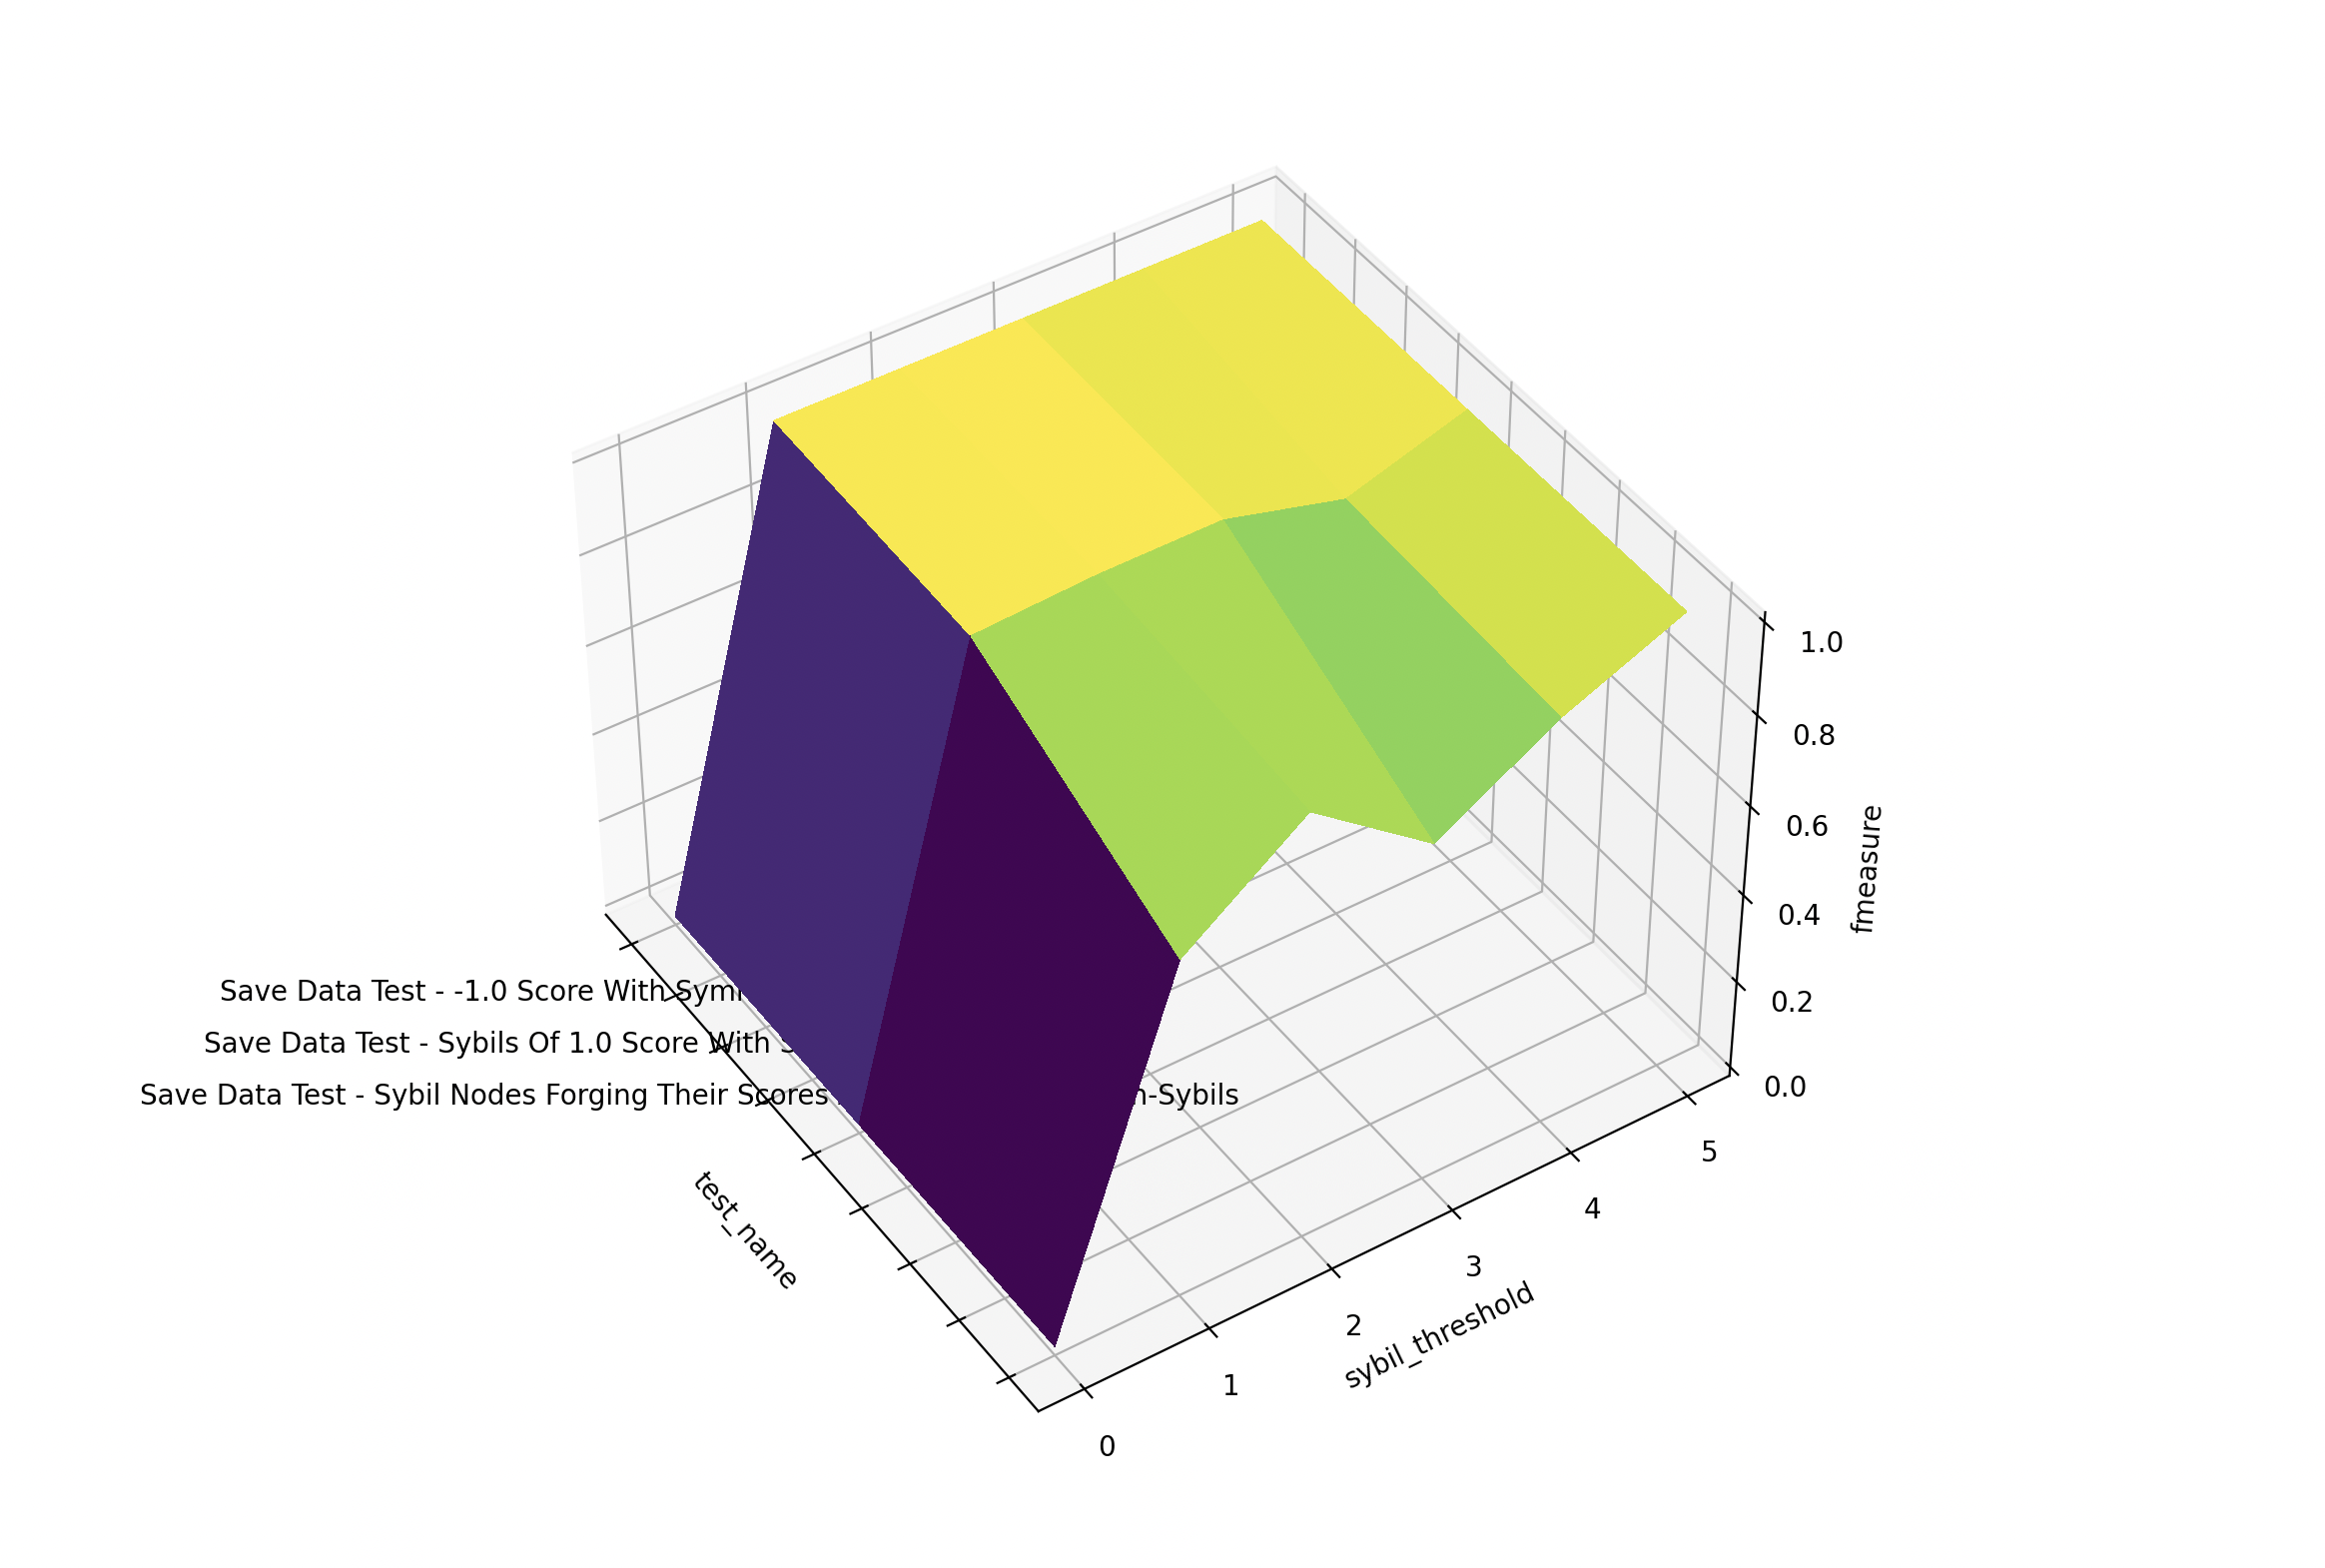
\includegraphics[width=\textwidth, height=\textwidth]{f-score-surface-plot}
\caption{F-scores by each attack type and sybil threshold}
\end{figure}

Here we have a surface plot of F-score according to attack and sybil threshold. As we can see, the most effective attack is for sybil nodes to self report scores of 0.0, yielding a minimum F-score of 0.73, the reduction here coming from false negatives. This is still a solid score for any classifier and compared to existing consensus models (i.e. Bitcoin) which has an F-score of 0 for sybil percentages above 50 percent (due to the fact that one outcome of a $51\%$ attack is removal of non-sybil nodes), is remarkably successful and provides a huge comparative advantage.


\begin{figure}
\centering
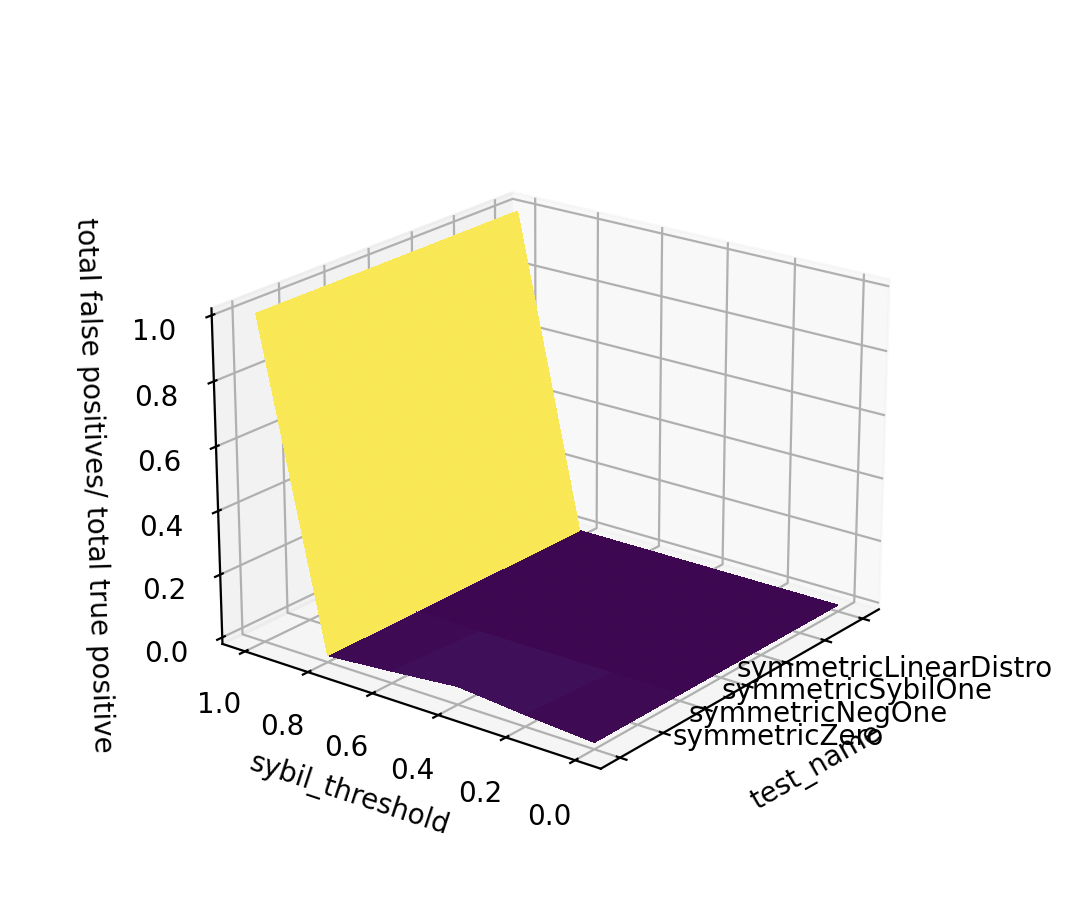
\includegraphics[width=\textwidth, height=\textwidth]{false-pos-vs-true-pos}
\caption{False positive / true positive by each attack type and sybil threshold}
\end{figure}

Here we have a plot of false positives / true positives. As mentioned above, F-scores drop primarily due to false negatives. However for our model which is most focused on removing sybil nodes, we can see that very few are not removed; specifically the small bump in symmetricZeroSybil has a maximum of 0.035, meaning only $3.5\%$ of nodes selected are from the sybil group. The spike at the end is the $100\%$ sybil case, which is where the model breaks down (note the actual was 1/0, so a value of 1.0 was imputed.)



\begin{figure}
\centering
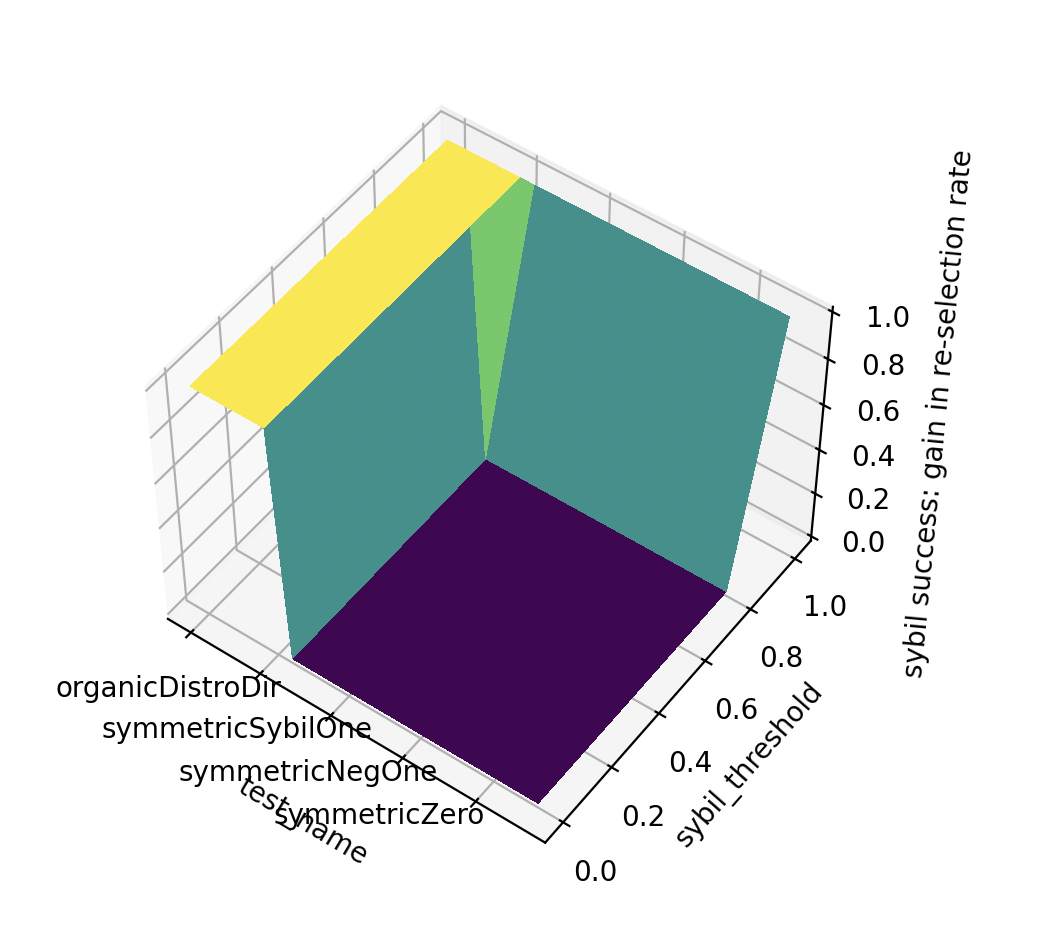
\includegraphics[width=\textwidth, height=\textwidth]{attack-success-suface-plot}
\caption{Sybil node gain}
\end{figure}

Here we have a plot of the difference between nodes cheating and not cheating. The vertical axis is the percent increase in sybil nodes (forging scores) that are selected for the next round of consensus vs if they actually just submitted scores based upon their true entropy rate (not cheating). The ledge on the top left represents the perfect non-sybil case ($0\%$) and the top right shows the $100\%$ sybil case; both of these shows $100\%$ of nodes selected for next round (as expected). Most importantly, the flat plane shows that the only sybil nodes selected would have been selected anyway, based upon their immutable entropy rate; this means that the classifier removes gains from cheating.

\section{Sybil resistance}
Open networks pose inherent security risks deriving from Sybil attacks; where a group of individuals attempt to forge network or ledger state. The attack surface grows as the cost for participation, either through hash power or stake, is reduced; essentially reducing the cost of a sybil attack by minimizing the cost to run sybil nodes. This has the transitive effect of also reducing the efficacy of horizontal scaling techniques, which increase speed as a function of the number of nodes. 2MEME mitigates these attacks in such a way that promotes participation (low fees and high transactions per second), both as a miner and a user. 

\subsection{Sybil attack}
As shown in the false positive vs true positive plot, the classifier is able to remove the vast majority of sybil nodes (at most a $3.5\%$ sybil rate) and only fails with close to $100\%$ sybil rate. That being said, given that the size of the active peers is much less than the passive, it would be feasible, albeit of a low probability, that entire committees of active nodes could be sybil. However, our approach is still able to increase the cost required for a $100\%$ successful sybil attack beyond the typical $51\%$. 

Active L0 nodes are chosen from two buckets: the smallest set of nodes who's stake adds up to a minimum of $50\%$ and the rest of the nodes. Because of this, the cost to achieve a sybil attack with $100\%$ guarantee (i.e. all active nodes are sybil) would require over $50\%$ of the total stake in the network and over $50\%$ of the total hash power (number of nodes); most permissionless networks require only one of these to be over $50\%$ to fail whereas this system requires both.

Consider the case where $10\%$ of all L0 nodes contain over $50\%$ of staked tokens and the other $90\%$ makes up less than $50\%$, that would mean a guaranteed attack requires over $50\%$ of staked tokens and up to $100\%$ of the hash power. This is considerably more costly than pure POW or POS which fail above $50\%$ controlling hash power or stake, respectively.

\subsection{Lie and wait attack}
In a reputation system, a lie in wait attack occurs when nodes increase their reputation so that it can then use the high score later for abuse. In 2MEME, reputation is calculated based on an immutable log of information gain for each system, however the specific reputation score only has relevance within the context of the information gain of all other nodes and is ephemeral. Thus due to the nature of the model, which doesn't carry over reputation values between the active/passive cycle, it's not possible to 'save up reputation points' and spend them on an attack.

The closest one could come to this attack is performing well by producing minimal entropy in every snapshot throughout the entire consensus round, and then forging their score proposals, however this is the focus of the various attacks in the experimental analysis section and the model has shown to be successful at identifying sybil nodes regardless of their scores, or the distribution of scores across all sybil nodes.

\subsection{Eclipse attack}
As shown in the $L\Omega$ definition, the result of a $51\%$ attack is a network partition where the offending nodes would only have an invalid chain state. This is essentially how one would perform an Eclipse attack, where offending nodes send incorrect peer data or chain data to a newly joining node. In this case, honest nodes would not be able to join the invalid partition (validation of the download step from a sybil node would not pass) and honest subscribers such as client utilities or L2 applications would be able to identify a sybil partition via invalid published snapshots. The end result of a wider $51\%$ attack would be an increase in latency (as for an ordinary network partition) as opposed to an invalid chain state.


\section{Further investigation}
	Modifications to the self-avoiding walk implementation could yield positive effects. As in many Monte Carlo integrations, the direction chosen at each step could be chosen according to a distance metric as opposed to randomly. Albeit, at the computational cost of increasing the dimensionality of the trust graph’s edges as well as in-memory expense of the metric calculation. Notably, this approach was employed by N. Koroviako\footnote{https://www.sciencedirect.com/science/article/pii/S1877050912003936?ref=pdf\_download\&fr=RR-2\&rr=8306a2ef2866cee9} who used Jaccard similarity to define trust out of relationships between review texts; as 2MEME's approach focuses on information gain, it would follow to select the next path at each step based on minimizing entropy rate of second order proposals (each edge would contain raw proposals, and choose the next node that has the minimal entropy rate compared to the current’s proposals.)
	
	As our SAW has non-linear (fractal) dimensionality\footnote{http://www.math.uchicago.edu/~lawler/miami1.pdf}, another possible improvement could come from using Hausdorff clustering\footnote{https://arxiv.org/pdf/0801.0748.pdf} to identify embedded hierarchies (perfom classification in terms of the surface of clusters); this could have applications in further anomaly detection providing higher dimensions of entropy, which would be useful for improving the classifier with a differential equation solver or perhaps a graph embedding/deep learning approach. Note that the node influence metric calculated by the SAW is not strictly defined (it does not strictly obey the triangle equality, thus it's a measure not a metric) so it is actually compatible for the Hausdorff measure. 
	
	The cryptographic signatures described in the system architecture use ECDSA. However, with the dawn of quantum computers and the fact that elliptic curve cryptography is vulnerable Shor's algorithm\footnote{https://arxiv.org/pdf/1804.00200.pdf} new 'post-quantum' cryptography (PQC) has been introduced which would allow 2MEME to remain effective in a post-quantum world. Fortunately, due to the structure of the key utilities in our codebase, we can easily swap out ECDSA for these newer PQC implementations. 

	
\section{Conclusion}
It's been shown that 2MEME incentivizes consistency by rewarding nodes according to their information gain. Also by showing a lack of gain for sybil nodes while still minimizing removal of non-sybil nodes (as evidenced by the F-score distributions,) 2MEME is able to provide a fair playing field for honest nodes.
	
	
\end{document}
